\chapter{Manual de usuario}

\section{Introducción}

Sevillaneando es una aplicación móvil orientada al descubrimiento de eventos culturales y de ocio en Sevilla, con especial interés en dar visibilidad a propuestas emergentes o menos conocidas. Su finalidad no es únicamente mostrar un catálogo de actividades, sino ofrecer al usuario una experiencia completa de exploración, interacción y personalización a partir de sus intereses, su ubicación y su comportamiento dentro de la plataforma.

La aplicación permite consultar eventos, filtrarlos, localizarlos sobre el mapa, guardar aquellos que resulten de interés, apuntarse a ellos, compartirlos, valorarlos y participar en espacios de comunicación asociados. Además, incorpora funcionalidades avanzadas, como recomendaciones personalizadas y generación de rutas, que ayudan al usuario a descubrir nuevas actividades ajustadas a sus preferencias y a planificar mejor su asistencia.

Desde el punto de vista de uso, el sistema contempla distintos perfiles. El rol de usuario permite crear actividades. Por su parte, los roles de moderador y administrador cubren necesidades de supervisión y gestión interna de la aplicación.

El objetivo de este manual es guiar al usuario en el uso de la aplicación, describiendo sus principales entidades, requisitos de uso y flujos de interacción más relevantes. A lo largo del documento se explica cómo utilizar las distintas funcionalidades del sistema de manera progresiva, de forma que cualquier persona pueda comprender el funcionamiento general de la aplicación y aprovechar todas sus posibilidades.

\section{Definición de entidades y funcionalidades}

\begin{tcolorbox}[title=\textbf{Evento}]
El evento es la entidad principal del sistema y representa cada actividad cultural o de ocio disponible en la aplicación. Cada evento dispone de información descriptiva y funcional suficiente para que el usuario pueda decidir si le interesa asistir, guardarlo para más adelante o interactuar con él.

\vspace{0.4em}
\textbf{Funcionalidades}
\begin{itemize}[leftmargin=1.5em]
\item Creación de eventos públicos y privados.
\item Edición de la información del evento, como fecha, ubicación, descripción o precio.
\item Inscripción de usuarios.
\item Apertura de la ubicación del evento en aplicaciones externas de mapas.
\item Guardado del evento para consultas posteriores.
\item Visualización de asistentes.
\item Valoración del evento.
\item Acceso al chat asociado al evento.
\item Compartición del evento mediante enlace.
\item Gestión de estados: activo, finalizado y en moderación.
\item Inclusión en distintos listados personalizados.
\end{itemize}
\end{tcolorbox}

\begin{tcolorbox}[title=\textbf{Mapa de eventos}]
El mapa de eventos permite representar visualmente la distribución geográfica de las actividades disponibles. Esta funcionalidad resulta especialmente útil para usuarios que desean localizar eventos cercanos o comparar rápidamente varias opciones en función de su ubicación.

\vspace{0.4em}
\textbf{Funcionalidades}
\begin{itemize}[leftmargin=1.5em]
\item Visualización de eventos sobre mapa interactivo.
\item Clasificación aproximada por distancia mediante colores (verde, amarillo y rojo).
\item Configuración del radio de búsqueda.
\item Acceso directo al detalle del evento.
\item Uso de la ubicación del usuario como referencia.
\end{itemize}
\end{tcolorbox}

\begin{tcolorbox}[title=\textbf{Recomendaciones}]
El sistema de recomendaciones tiene como propósito adaptar la experiencia de uso a cada usuario. Para ello, tiene en cuenta factores como los intereses del perfil, la cercanía, las interacciones previas y otra información relevante del comportamiento dentro de la aplicación.

\vspace{0.4em}
\textbf{Funcionalidades}
\begin{itemize}[leftmargin=1.5em]
\item Recomendación de eventos según intereses del perfil.
\item Aprendizaje basado en la interacción del usuario.
\item Influencia de proximidad, valoraciones (propias y media global), eventos guardados, eventos apuntados, eventos vistos, eventos compartidos. .
\item Consideración de fechas y disponibilidad.
\item Generación de rutas recomendadas.
\end{itemize}
\end{tcolorbox}

\begin{tcolorbox}[title=\textbf{Perfil de usuario}]
El perfil recoge la información personal y las preferencias del usuario. Esta entidad resulta fundamental, ya que condiciona parte del comportamiento personalizado del sistema, especialmente en lo relativo a recomendaciones y funciones basadas en ubicación.

\vspace{0.4em}
\textbf{Funcionalidades}
\begin{itemize}[leftmargin=1.5em]
\item Edición de datos personales.
\item Configuración de ubicación.
\item Gestión de intereses (categorías preferidas).
\item Cambio de contraseña.
\item Eliminación de cuenta.
\end{itemize}
\end{tcolorbox}

\begin{tcolorbox}[title=\textbf{Rutas}]
Las rutas son agrupaciones de eventos organizadas para facilitar la planificación del usuario. Pueden responder tanto a una lógica automática de recomendación como a la creación manual por parte de los propios usuarios. Este es otro punto clave, ya que permite agrupar eventos relacionados de forma coherente y optimizada en función de factores como la ubicación, el horario y las preferencias del usuario. De este modo, no solo se facilita la planificación de la asistencia a múltiples eventos, sino que también se incrementa la visibilidad de eventos relevantes que podrían pasar desapercibidos de forma individual, mejorando así el descubrimiento de contenido y la eficiencia en la experiencia de uso.

\vspace{0.4em}
\textbf{Funcionalidades}
\begin{itemize}[leftmargin=1.5em]
\item Generación automática de rutas recomendadas.
\item Creación manual de rutas por usuarios.
\item Optimización por distancia y horarios.
\item Consulta y valoración de rutas creadas por otros usuarios.
\end{itemize}
\end{tcolorbox}

\begin{tcolorbox}[title=\textbf{Notificaciones}]
El sistema de notificaciones mantiene informado al usuario sobre sucesos relevantes ocurridos dentro de la aplicación. Gracias a este módulo, la plataforma puede comunicar cambios de estado, recordatorios y eventos cercanos de forma proactiva.

\vspace{0.4em}
\textbf{Funcionalidades}
\begin{itemize}[leftmargin=1.5em]
\item Notificación de aprobación o rechazo de eventos.
\item Recordatorios previos a eventos apuntados.
\item Avisos sobre eventos cercanos según la ubicación.
\end{itemize}
\end{tcolorbox}

\begin{tcolorbox}[title=\textbf{Mensajería}]
Sistema de comunicación entre usuarios. Este módulo resulta fundamental dentro de la aplicación, ya que facilita la interacción directa entre participantes de un mismo evento o usuarios con intereses comunes. Gracias a esta funcionalidad, se promueve la conexión social, permitiendo coordinar asistencia, resolver dudas y organizar encuentros previos o durante el evento. Además, contribuye a mejorar la experiencia del usuario al fomentar la colaboración, la planificación compartida y la creación de redes sociales dentro de la plataforma.

\vspace{0.4em}
\textbf{Funcionalidades}
\begin{itemize}[leftmargin=1.5em]
\item Chat asociado a eventos.
\item Mensajes privados.
\item Acceso desde asistentes o perfiles de usuario.
\item Envío de texto e imágenes.
\end{itemize}
\end{tcolorbox}

\begin{tcolorbox}[title=\textbf{Administración}]
La administración cubre las funciones de gestión global de la plataforma reservadas al rol de administrador.

\vspace{0.4em}
\textbf{Funcionalidades}
\begin{itemize}[leftmargin=1.5em]
\item Gestión de usuarios y roles.
\item Gestión de categorías.
\end{itemize}
\end{tcolorbox}

\begin{tcolorbox}[title=\textbf{Moderación}]
La moderación se ocupa de supervisar los contenidos que deben ser validados antes de su publicación, con el objetivo de mantener la coherencia y fiabilidad del sistema.

\vspace{0.4em}
\textbf{Funcionalidades}
\begin{itemize}[leftmargin=1.5em]
\item Revisión de eventos pendientes.
\item Edición previa a la publicación.
\item Aprobación o rechazo de eventos.
\end{itemize}
\end{tcolorbox}

\section{Requisitos técnicos}

Para utilizar correctamente la aplicación es necesario disponer de los siguientes elementos:

\begin{itemize}[leftmargin=1.5em]
\item Un dispositivo móvil compatible con iOS o Android.
\item Conexión a Internet, ya sea mediante WiFi o datos móviles.
\item Una cuenta de correo electrónico válida para el registro y recuperación de contraseña.
\item Permisos recomendados de acceso a cámara y galería, necesarios para funcionalidades de imagen.
\item Permisos de ubicación, recomendables para el uso del mapa y la recepción de notificaciones cercanas.
\end{itemize}

\section{Guía de uso de la aplicación}

Una vez definidas las entidades principales del sistema, en esta sección se describe el uso práctico de la aplicación desde la perspectiva del usuario. El objetivo no es únicamente enumerar pantallas, sino explicar cómo puede utilizarse la plataforma para cubrir necesidades reales, como descubrir eventos, organizar la asistencia, comunicarse con otros usuarios o gestionar actividades propias.

\clearpage

\subsection{Registro e inicio de sesión (para todos los roles)}

El primer paso para utilizar la aplicación consiste en crear una cuenta. Para ello, el usuario debe completar el formulario de registro con sus datos básicos. Aunque la plataforma contempla distintos roles, el proceso de alta está pensado para cuentas de usuario estándar, siendo el administrador principal el que decide cuantos moderadores y administradores se añaden. Para solicitar cualquier cambio en la aplicación, váyase al correo que se muestra en la página de inicio al final de ella.

Una vez creada la cuenta, el acceso al sistema se realiza desde la pantalla de inicio de sesión. En caso de no recordar la contraseña, la aplicación ofrece una funcionalidad de recuperación mediante correo electrónico.

\bigskip

\textbf{Aspectos a tener en cuenta:}
\begin{itemize}[leftmargin=1.5em]
\item El correo electrónico debe ser válido.
\item La contraseña debe recordarse o recuperarse mediante el correo asociado.
\item El registro crea cuentas con rol de usuario.
\end{itemize}

\begin{figure}[H]
    \centering
    \begin{subfigure}{0.35\linewidth}
        \centering
        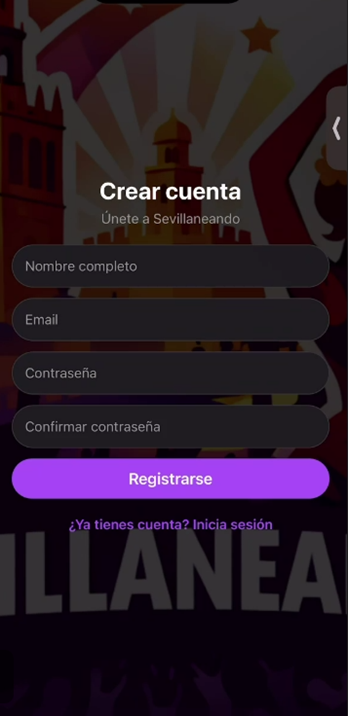
\includegraphics[width=\linewidth]{figures/paso1/crear_cuenta.png}
        \caption{Crear cuenta}
    \end{subfigure}
    \hspace{0.1\linewidth}
    \begin{subfigure}{0.35\linewidth}
        \centering
        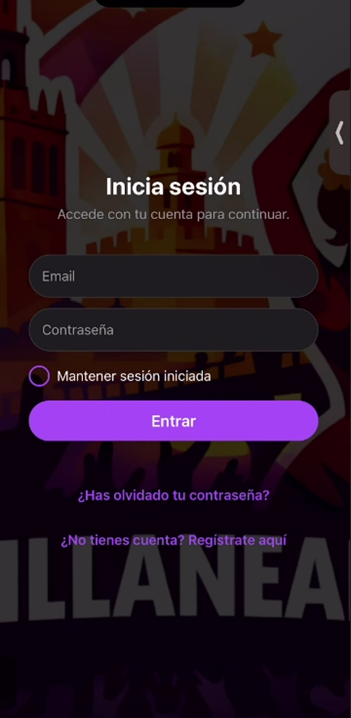
\includegraphics[width=\linewidth]{figures/paso1/iniciar_sesion.png}
        \caption{Iniciar sesión}
    \end{subfigure}
    \caption{Acceso a la aplicación}
\end{figure}

\clearpage

\subsection{Gestión del perfil (para todos los roles)}

Tras iniciar sesión, el usuario puede acceder al menú lateral desde la esquina superior izquierda. Desde este menú se accede a la gestión del perfil, al cambio de tema visual y al cierre de sesión.

La pantalla de perfil permite editar la información personal del usuario, como la foto, el nombre de usuario, el correo electrónico, la ubicación y los intereses. Esta información no solo tiene valor identificativo, sino que influye en otras funciones del sistema. En particular, la ubicación permite habilitar el mapa y los filtros de cercanía, mientras que los intereses resultan relevantes para las recomendaciones.

También desde esta sección pueden realizarse acciones sensibles, como el cambio de contraseña o la eliminación de la cuenta.

\bigskip

\textbf{Validaciones y recomendaciones:}
\begin{itemize}[leftmargin=1.5em]
\item Se recomienda indicar una ubicación para habilitar todas las funciones de proximidad.
\item Los datos modificados deben guardarse correctamente antes de salir.
\item El correo electrónico debe mantener un formato válido.
\end{itemize}

\begin{figure}[H]
    \centering
    \begin{subfigure}{0.285\linewidth}
        \centering
        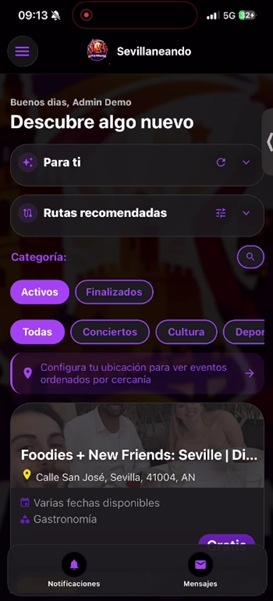
\includegraphics[width=\linewidth]{figures/home_screen.png}
        \caption{Página principal}
    \end{subfigure}
    \hspace{0.02\linewidth}
    \begin{subfigure}{0.3\linewidth}
        \centering
        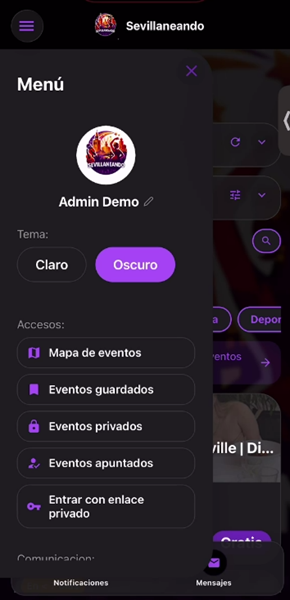
\includegraphics[width=\linewidth]{figures/lateral_menu.png}
        \caption{Menú lateral}
    \end{subfigure}
    \hspace{0.02\linewidth}
    \begin{subfigure}{0.29\linewidth}
        \centering
        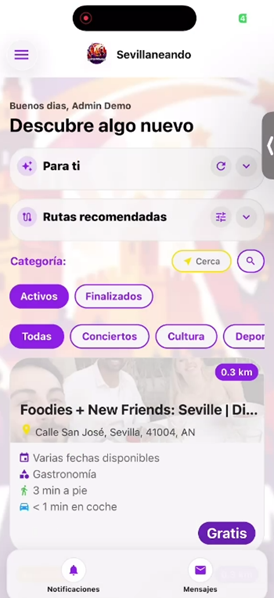
\includegraphics[width=\linewidth]{figures/paso2/modo_claro.png}
        \caption{Modo claro}
    \end{subfigure}
    \caption{Acceso y opciones del perfil}
\end{figure}

\begin{figure}[H]
    \centering
    \begin{subfigure}{0.33\linewidth}
        \centering
        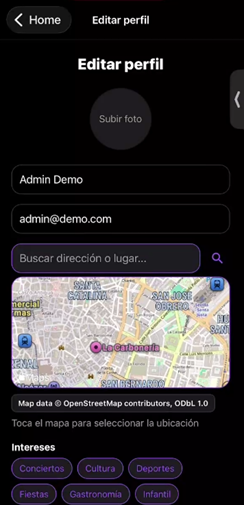
\includegraphics[width=\linewidth]{figures/paso2/edit_profile.png}
        \caption{Editar perfil 1}
    \end{subfigure}
    \hspace{0.02\linewidth}
    \begin{subfigure}{0.33\linewidth}
        \centering
        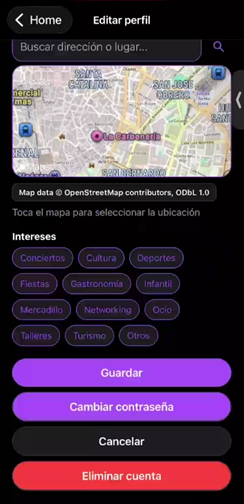
\includegraphics[width=\linewidth]{figures/paso2/edit_profile2.png}
        \caption{Editar perfil 2}
    \end{subfigure}
    \hspace{0.02\linewidth}
    \begin{subfigure}{0.34\linewidth}
        \centering
        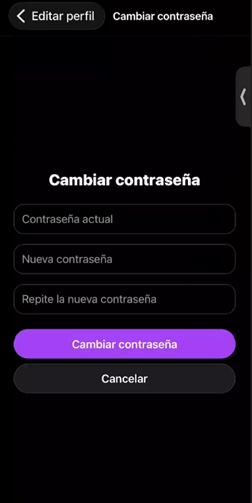
\includegraphics[width=\linewidth]{figures/paso2/edit_profile3.png}
        \caption{Cambiar contraseña}
    \end{subfigure}
    \caption{Gestión del perfil}
\end{figure}

\clearpage

\subsection{Mapa de eventos (para todos los roles)}

La aplicación permite consultar los eventos en un mapa interactivo, lo que resulta útil para usuarios que desean localizar actividades próximas a su ubicación. Esta funcionalidad se encuentra accesible desde el menú lateral.

Los eventos se representan visualmente mediante colores, que permiten identificar de forma rápida si se encuentran más cerca o más lejos del usuario, siendo el verde los más cercanos y el rojo los más lejanos. Además, puede ajustarse el radio de búsqueda para adaptar el mapa a las preferencias de exploración.

Cuando el usuario selecciona un evento dentro del mapa, se muestra una vista resumida del mismo. Si vuelve a pulsar sobre él, accede a la pantalla de detalle.

\bigskip

\textbf{Aspectos a tener en cuenta:}
\begin{itemize}[leftmargin=1.5em]
\item Es necesario haber configurado una ubicación previamente en el perfil.
\end{itemize}

\begin{figure}[H]
    \centering
    \begin{subfigure}{0.3\linewidth}
        \centering
        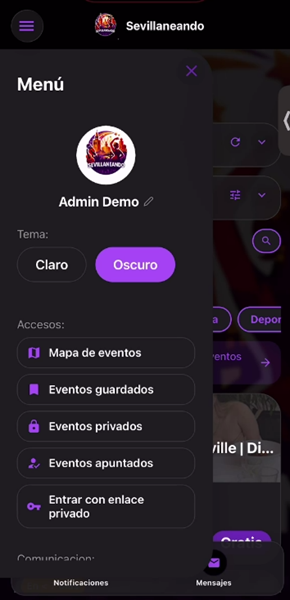
\includegraphics[width=\linewidth]{figures/lateral_menu.png}
        \caption{Menú lateral}
    \end{subfigure}
    \hspace{0.01\linewidth}
    \begin{subfigure}{0.293\linewidth}
        \centering
        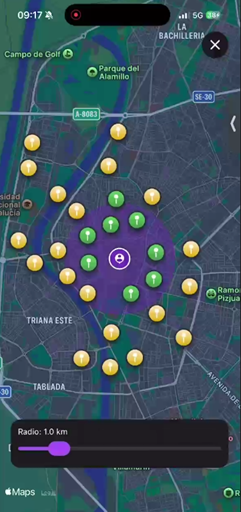
\includegraphics[width=\linewidth]{figures/paso3/mapa1.png}
        \caption{Eventos en el mapa}
    \end{subfigure}
    \hspace{0.01\linewidth}
    \begin{subfigure}{0.29\linewidth}
        \centering
        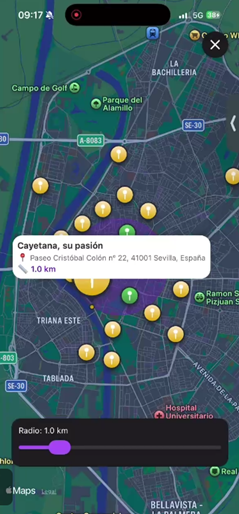
\includegraphics[width=\linewidth]{figures/paso3/mapa2.png}
        \caption{Etiqueta del evento}
    \end{subfigure}
    \caption{Mapa de eventos}
\end{figure}

\clearpage

\subsection{Página principal y filtros (para todos los roles)}

La página principal es el espacio central de consulta de la aplicación. En ella se muestra el listado general de eventos disponibles y una serie de mecanismos de búsqueda y filtrado que permiten al usuario localizar actividades según distintos criterios.

Desde esta vista pueden diferenciarse eventos activos y finalizados. También es posible filtrar por categoría, utilizar el buscador avanzado y aplicar filtros de cercanía cuando se dispone de ubicación configurada. Este conjunto de filtros facilita una exploración más precisa de la oferta disponible.

\bigskip

\textbf{Aspectos a tener en cuenta:}
\begin{itemize}[leftmargin=1.5em]
\item Los eventos finalizados siguen siendo visibles, pero no admiten inscripción.
\item El filtrado por cercanía requiere ubicación.
\item Las categorías pueden organizarse arrastándolas horizontalmente para dejar primero las favoritas.
\end{itemize}

\begin{figure}[H]
    \centering
    \begin{subfigure}{0.3\linewidth}
        \centering
        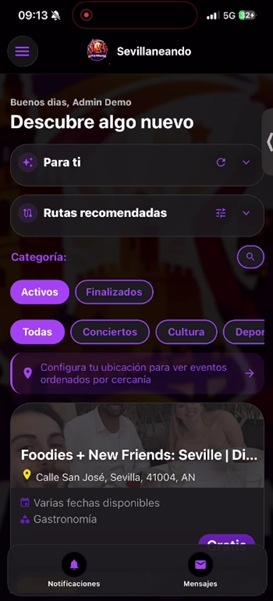
\includegraphics[width=\linewidth]{figures/home_screen.png}
        \caption{Página principal}
    \end{subfigure}
    \hspace{0.01\linewidth}
    \begin{subfigure}{0.324\linewidth}
        \centering
        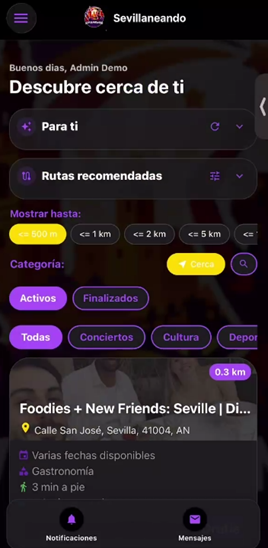
\includegraphics[width=\linewidth]{figures/paso4/cerca.png}
        \caption{Búsqueda por cercanía}
    \end{subfigure}
    \hspace{0.01\linewidth}
    \begin{subfigure}{0.321\linewidth}
        \centering
        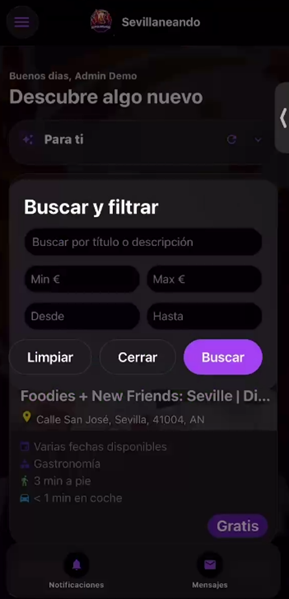
\includegraphics[width=\linewidth]{figures/paso4/busqueda.png}
        \caption{Buscador avanzado}
    \end{subfigure}
    \caption{Filtros de búsqueda}
\end{figure}

\clearpage

\subsection{Detalle de evento}

La pantalla de detalle de un evento reúne toda la información necesaria para que el usuario pueda valorar si desea asistir o interactuar con la actividad. Se trata de una de las vistas más importantes de la aplicación, ya que desde ella se ejecutan muchas de las acciones principales del sistema.

Entre las operaciones disponibles se encuentran abrir la ubicación en una aplicación de mapas externa, apuntarse al evento, consultar asistentes, guardarlo, compartirlo o valorarlo. Además, desde esta misma vista puede abrirse el chat del evento para enviar mensajes o imágenes, y pulsando sobre estos se podrán eliminar.

Las acciones realizadas en esta pantalla tienen un efecto directo en el comportamiento personalizado del sistema, ya que alimentan procesos como las recomendaciones o la generación de rutas.

\bigskip

\textbf{Aspectos a tener en cuenta:}
\begin{itemize}[leftmargin=1.5em]
\item Algunas acciones solo están disponibles en eventos activos (inscribirse) y públicos (compartir).
\item La interacción con el evento influye en futuras recomendaciones.
\item Desde asistentes y perfiles del chat puede iniciarse mensajería privada.
\end{itemize}

\begin{figure}[H]
    \centering
    \begin{subfigure}{0.3\linewidth}
        \centering
        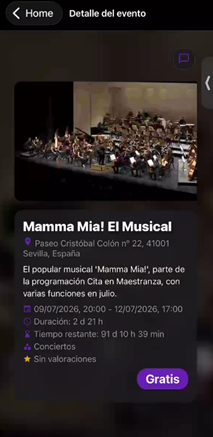
\includegraphics[width=\linewidth]{figures/paso5/event_detail.png}
        \caption{Detalles del evento}
    \end{subfigure}
    \hspace{0.02\linewidth}
    \begin{subfigure}{0.305\linewidth}
        \centering
        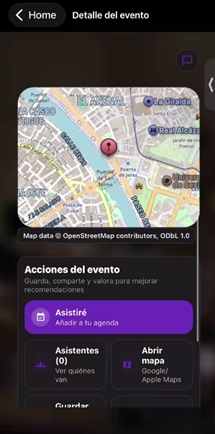
\includegraphics[width=\linewidth]{figures/paso5/event_detail2.png}
        \caption{Detalles del evento 2}
    \end{subfigure}
    \hspace{0.02\linewidth}
    \begin{subfigure}{0.306\linewidth}
        \centering
        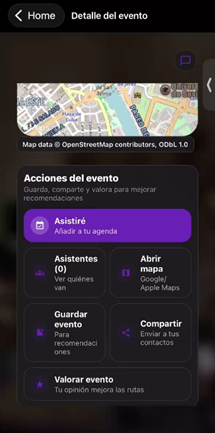
\includegraphics[width=\linewidth]{figures/paso5/event_detail3.png}
        \caption{Acciones del evento}
    \end{subfigure}
    \caption{Pantalla del evento}
\end{figure}

\begin{figure}[H]
    \centering
    \begin{subfigure}{0.35\linewidth}
        \centering
        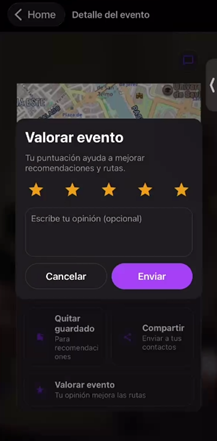
\includegraphics[width=\linewidth]{figures/paso5/valoracion.png}
        \caption{Valorar evento}
    \end{subfigure}
    \hspace{0.02\linewidth}
    \begin{subfigure}{0.352\linewidth}
        \centering
        
\includegraphics[width=\linewidth]{figures/paso5/chat_evento.png}
        \caption{Chat del evento}
    \end{subfigure}
    \caption{Interacción dentro del evento}
\end{figure}

\clearpage

\subsection{Listados de eventos}

La aplicación organiza determinados eventos en listados personalizados que facilitan su consulta posterior. Estos listados se encuentran accesibles desde el menú lateral y responden a diferentes tipos de interacción previa del usuario.

Entre ellos se encuentran los eventos guardados, los eventos a los que el usuario se ha apuntado y el calendario, donde se muestran aquellos que tienen fecha definida. Estos espacios facilitan la planificación y el seguimiento de actividades de interés.

\begin{figure}[H]
    \centering
    \begin{subfigure}{0.35\linewidth}
        \centering
        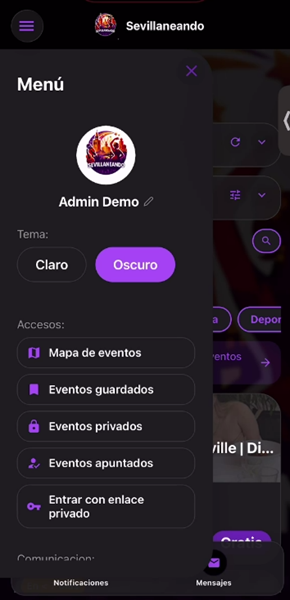
\includegraphics[width=\linewidth]{figures/lateral_menu.png}
        \caption{Menú lateral}
    \end{subfigure}
    \hspace{0.1\linewidth}
    \begin{subfigure}{0.35\linewidth}
        \centering
        
\includegraphics[width=\linewidth]{figures/paso6/eventos_apuntados.png}
        \caption{Eventos guardados}
    \end{subfigure}
    \caption{Listado de eventos guardados}
\end{figure}

\begin{figure}[H]
    \centering
    \begin{subfigure}{0.3\linewidth}
        \centering
        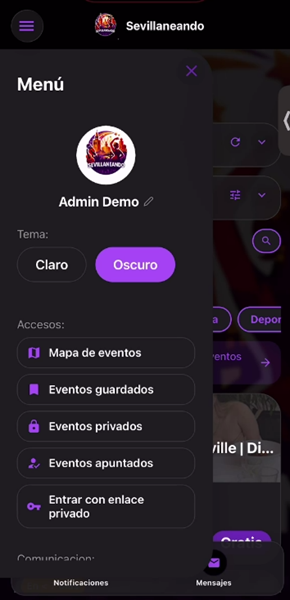
\includegraphics[width=\linewidth]{figures/lateral_menu.png}
        \caption{Menú lateral}
    \end{subfigure}
    \hspace{0.1\linewidth}
    \begin{subfigure}{0.3\linewidth}
        \centering
        
\includegraphics[width=\linewidth]{figures/paso6/eventos_apuntados.png}
        \caption{Eventos apuntados}
    \end{subfigure}
    \caption{Listado de eventos apuntados}
\end{figure}

\begin{figure}[H]
    \centering
    \begin{subfigure}{0.3\linewidth}
        \centering
        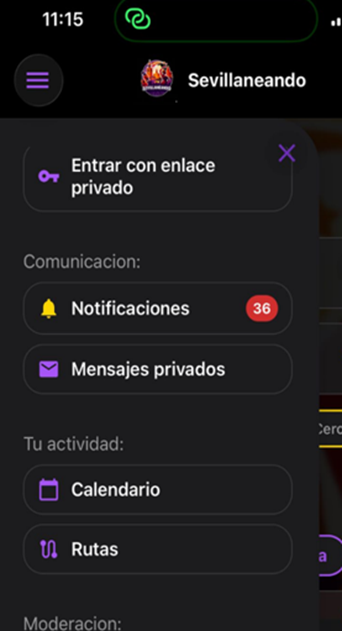
\includegraphics[width=\linewidth]{figures/paso6/lateral_menu2.png}
        \caption{Menú lateral}
    \end{subfigure}
    \hspace{0.1\linewidth}
    \begin{subfigure}{0.26\linewidth}
        \centering
        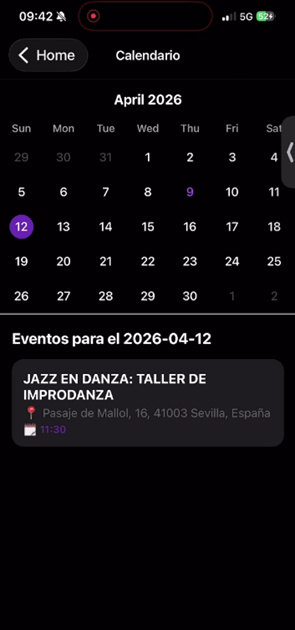
\includegraphics[width=\linewidth]{figures/paso6/calendario.png}
        \caption{Calendario}
    \end{subfigure}
    \caption{Calendario de eventos}
\end{figure}

\clearpage

\subsection{Gestión de administrador (rol de administrador)}

El rol de administrador dispone de funcionalidades específicas para mantener la organización global del sistema. Estas funciones se encuentran disponibles desde el menú lateral y se orientan a la gestión de usuarios y categorías.

En el panel de administración pueden modificarse roles y eliminarse usuarios cuando sea necesario. Además, existe una pantalla específica para la creación, edición y eliminación de categorías, fundamentales para la clasificación de eventos y preferencias.

\bigskip

\textbf{Credenciales de prueba:}
\begin{itemize}[leftmargin=1.5em]
\item Email: \texttt{admin@demo.com}
\item Contraseña: \texttt{administrador}
\end{itemize}

\begin{figure}[H]
    \centering
    \begin{subfigure}{0.30\linewidth}
        \centering
        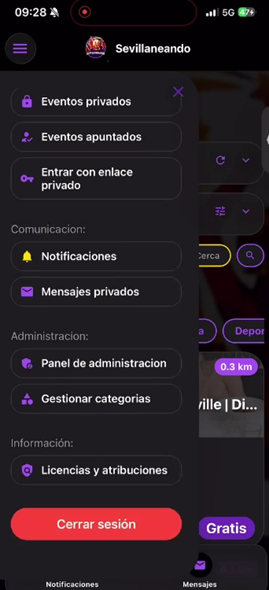
\includegraphics[width=\linewidth]{figures/paso7/menu_admin.png}
        \caption{Menú de administrador}
    \end{subfigure}
    \hspace{0.02\linewidth}
    \begin{subfigure}{0.312\linewidth}
        \centering
        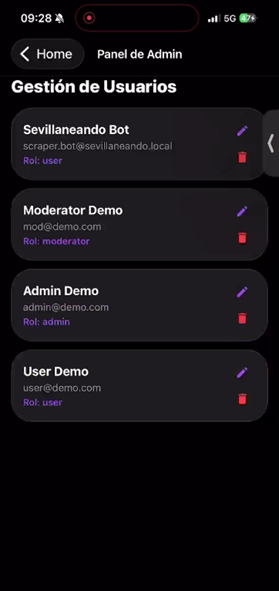
\includegraphics[width=\linewidth]{figures/paso7/panel_admin.png}
        \caption{Gestión de usuarios}
    \end{subfigure}
    \hspace{0.02\linewidth}
    \begin{subfigure}{0.31\linewidth}
        \centering
        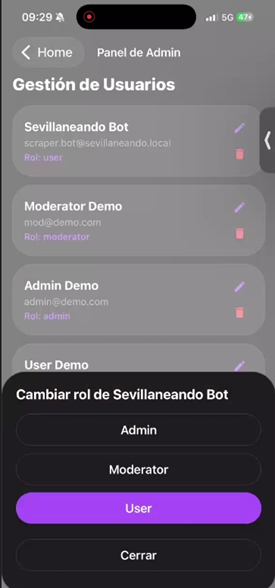
\includegraphics[width=\linewidth]{figures/paso7/edit_user.png}
        \caption{Editar usuario}
    \end{subfigure}
    \caption{Funcionalidades de administración}
\end{figure}

\begin{figure}[H]
    \centering
    \begin{subfigure}{0.332\linewidth}
        \centering
        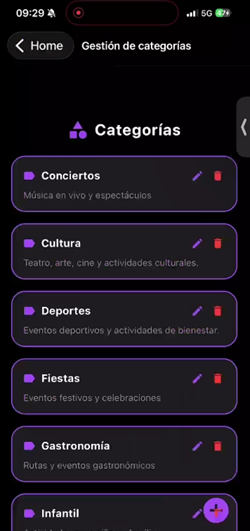
\includegraphics[width=\linewidth]{figures/paso7/gest_categ.png}
        \caption{Categorías}
    \end{subfigure}
    \hspace{0.02\linewidth}
    \begin{subfigure}{0.33\linewidth}
        \centering
        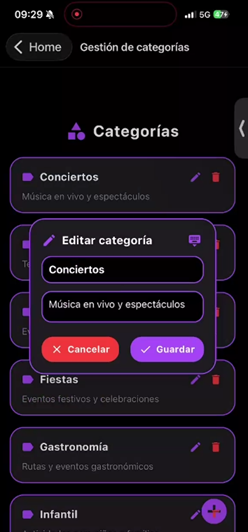
\includegraphics[width=\linewidth]{figures/paso7/edit_category.png}
        \caption{Editar categoría}
    \end{subfigure}
    \hspace{0.02\linewidth}
    \begin{subfigure}{0.328\linewidth}
        \centering
        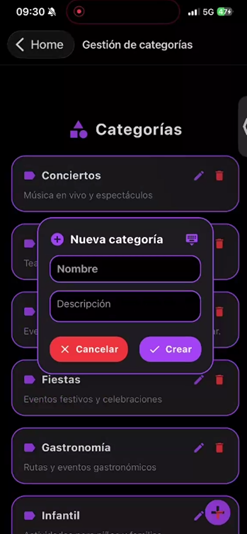
\includegraphics[width=\linewidth]{figures/paso7/crear_categ.png}
        \caption{Crear categoría}
    \end{subfigure}
    \caption{Gestión de categorías}
\end{figure}

\clearpage

\subsection{Recomendaciones y rutas recomendadas (para todos los roles)}

La página principal incorpora una sección personalizada en la que se muestran eventos recomendados y rutas sugeridas. Estas propuestas se generan a partir de factores como la distancia, las categorías preferidas, las interacciones previas del usuario y la valoración de los eventos.

Las rutas recomendadas, además, pueden configurarse mediante distintos ajustes, permitiendo adaptar su generación a determinadas preferencias del usuario.

\begin{figure}[H]
    \centering
    \begin{subfigure}{0.31\linewidth}
        \centering
        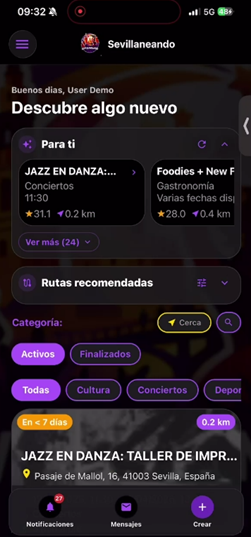
\includegraphics[width=\linewidth]{figures/paso8/recomendados.png}
        \caption{Recomendaciones}
    \end{subfigure}
    \hspace{0.01\linewidth}
    \begin{subfigure}{0.305\linewidth}
        \centering
        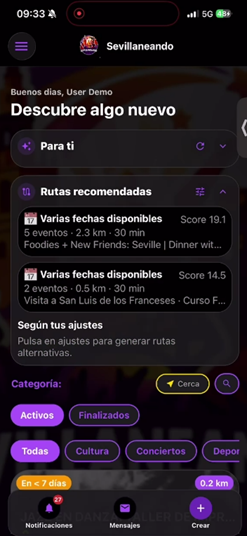
\includegraphics[width=\linewidth]{figures/paso8/rutas_recomendadas.png}
        \caption{Rutas recomendadas}
    \end{subfigure}
    \hspace{0.01\linewidth}
    \begin{subfigure}{0.302\linewidth}
        \centering
        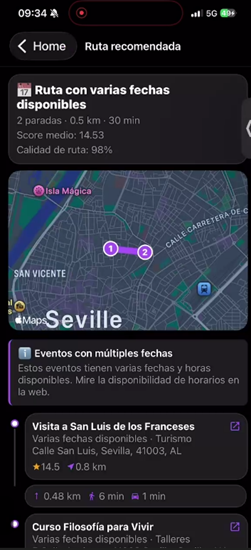
\includegraphics[width=\linewidth]{figures/paso8/detalles_ruta.png}
        \caption{Detalles de la ruta}
    \end{subfigure}
    \caption{Recomendaciones y rutas}
\end{figure}

\clearpage

\subsection{Rutas creadas por usuarios (para todos los roles)}

Además de las rutas generadas automáticamente por el sistema, la aplicación permite consultar y crear rutas manuales desde una sección específica del menú lateral. Estas rutas responden a experiencias o propuestas compartidas por otros usuarios y pueden ser valoradas por la comunidad.

Esta funcionalidad amplía la dimensión social y colaborativa del sistema, permitiendo que los usuarios recomienden recorridos ya experimentados y valorarlos.

\begin{figure}[H]
    \centering
    \begin{subfigure}{0.245\linewidth}
        \centering
        
\includegraphics[width=\linewidth]{figures/paso9/menu_lateral.png}
        \caption{Menú lateral}
    \end{subfigure}
    \hspace{0.02\linewidth}
    \begin{subfigure}{0.24\linewidth}
        \centering
        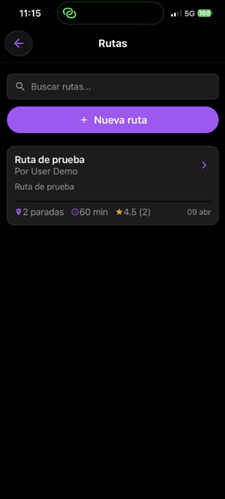
\includegraphics[width=\linewidth]{figures/paso9/rutas.png}
        \caption{Listado de rutas}
    \end{subfigure}
    \hspace{0.02\linewidth}
    \begin{subfigure}{0.245\linewidth}
        \centering
        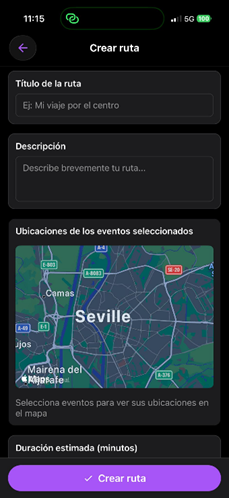
\includegraphics[width=\linewidth]{figures/paso9/crear_ruta.png}
        \caption{Crear ruta 1}
    \end{subfigure}

    \vspace{0.5cm}

    \begin{subfigure}{0.252\linewidth}
        \centering
        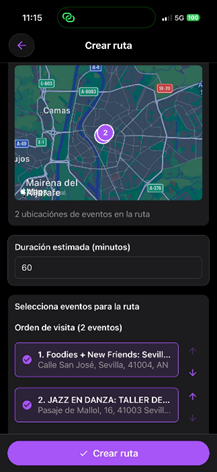
\includegraphics[width=\linewidth]{figures/paso9/crear_ruta2.png}
        \caption{Crear ruta 2}
    \end{subfigure}
    \hspace{0.02\linewidth}
    \begin{subfigure}{0.252\linewidth}
        \centering
        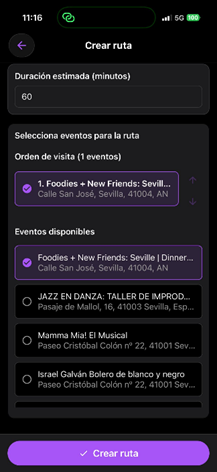
\includegraphics[width=\linewidth]{figures/paso9/crear_ruta3.png}
        \caption{Crear ruta 3}
    \end{subfigure}
    \hspace{0.02\linewidth}
    \begin{subfigure}{0.252\linewidth}
        \centering
        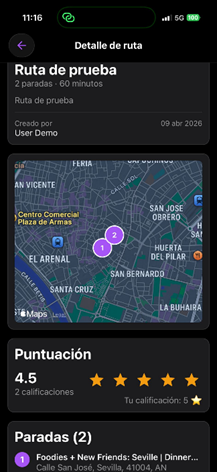
\includegraphics[width=\linewidth]{figures/paso9/detalle_ruta.png}
        \caption{Detalles de ruta}
    \end{subfigure}
    \caption{Rutas creadas por usuarios}
\end{figure}

\clearpage

\subsection{Creación de eventos (rol de usuario)}

Los usuarios pueden crear nuevos eventos desde la página principal o desde el menú lateral. Durante este proceso deben completar el formulario correspondiente con la información necesaria del evento.

La aplicación permite crear eventos privados, pensados para compartirse mediante enlace, y eventos públicos, cuya publicación dependerá del proceso de moderación.

\bigskip

\textbf{Aspectos a tener en cuenta:}
\begin{itemize}[leftmargin=1.5em]
\item Es recomendable completar todos los campos relevantes del formulario.
\item En eventos privados se genera un enlace de acceso compartible al que se tendrá que acceder para que sea visible.
\item En eventos públicos se requiere moderación antes de ser visibles para el resto.
\end{itemize}

\begin{figure}[H]
    \centering
    \begin{subfigure}{0.35\linewidth}
        \centering
        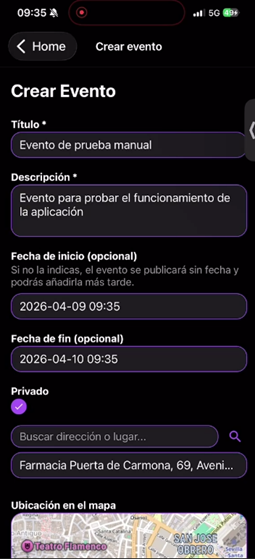
\includegraphics[width=\linewidth]{figures/paso10/crear_evento.png}
        \caption{Crear evento}
    \end{subfigure}
    \hspace{0.1\linewidth}
    \begin{subfigure}{0.356\linewidth}
        \centering
        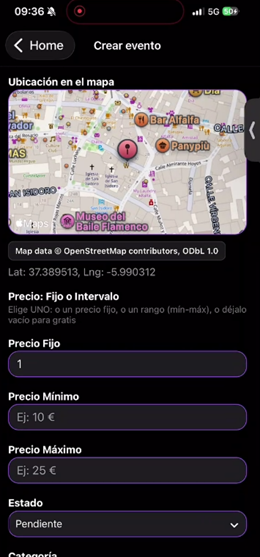
\includegraphics[width=\linewidth]{figures/paso10/crear_evento2.png}
        \caption{Crear evento 2}
    \end{subfigure}
    \caption{Creación de eventos}
\end{figure}

\begin{figure}[H]
    \centering
    \begin{subfigure}{0.35\linewidth}
        \centering
        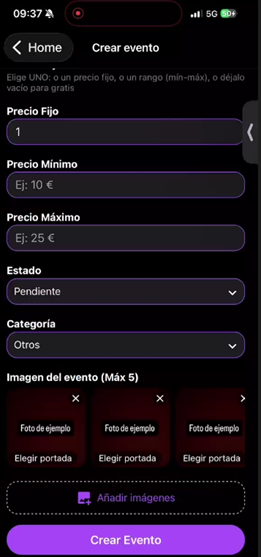
\includegraphics[width=\linewidth]{figures/paso10/crear_evento3.png}
        \caption{Crear evento 3}
    \end{subfigure}
    \hspace{0.1\linewidth}
    \begin{subfigure}{0.35\linewidth}
        \centering
        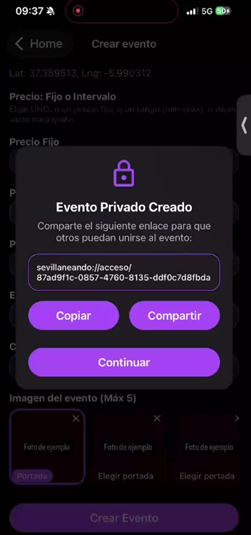
\includegraphics[width=\linewidth]{figures/paso10/evento_privado.png}
        \caption{Enlace privado}
    \end{subfigure}
    \caption{Creación de eventos }
\end{figure}

\clearpage

\subsection{Eventos privados (todos los roles)}

Los eventos privados están pensados para contextos en los que el acceso no debe ser abierto a todos los usuarios. Para participar en ellos, el usuario debe acceder mediante un enlace compartido por el creador.

Una vez introducido el enlace correspondiente, el evento pasa a formar parte del entorno visible para ese usuario. No obstante, este tipo de eventos mantiene restricciones específicas en cuanto a su difusión, siendo el creador el único que puede compartirlo.

\begin{figure}[H]
    \centering
    \begin{subfigure}{0.30\linewidth}
        \centering
        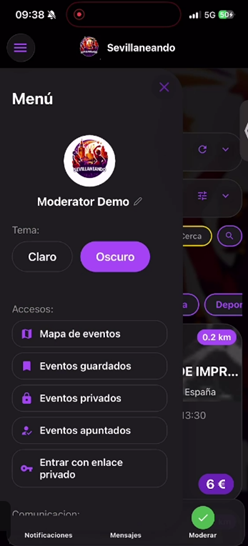
\includegraphics[width=\linewidth]{figures/paso11/menu_lateral.png}
        \caption{Menú lateral}
    \end{subfigure}
    \hspace{0.02\linewidth}
    \begin{subfigure}{0.308\linewidth}
        \centering
        
\includegraphics[width=\linewidth]{figures/paso11/evento_privado.png}
        \caption{Acceso privado}
    \end{subfigure}
    \hspace{0.02\linewidth}
    \begin{subfigure}{0.306\linewidth}
        \centering
        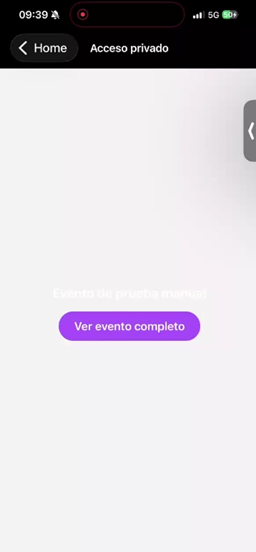
\includegraphics[width=\linewidth]{figures/paso11/evento_privado2.png}
        \caption{Ver evento privado}
    \end{subfigure}
    \caption{Acceso a evento privado}
\end{figure}

\begin{figure}[H]
    \centering
    \begin{subfigure}{0.358\linewidth}
        \centering
        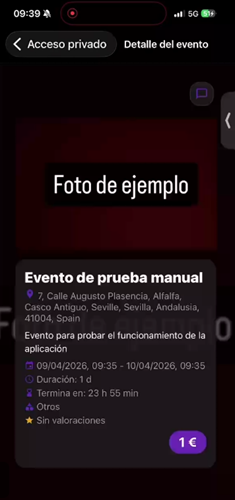
\includegraphics[width=\linewidth]{figures/paso11/detalles_event_priv.png}
        \caption{Evento privado}
    \end{subfigure}
    \hspace{0.02\linewidth}
    \begin{subfigure}{0.353\linewidth}
        \centering
        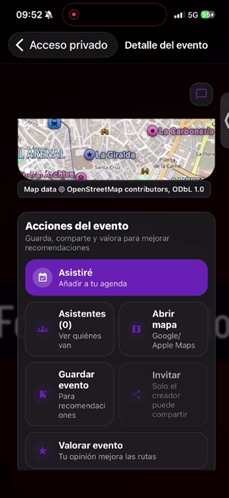
\includegraphics[width=\linewidth]{figures/paso11/det_ev_priv2.png}
        \caption{Evento privado 2}
    \end{subfigure}
    \caption{Consulta de evento privado}
\end{figure}

\clearpage

\subsection{Gestión de eventos privados (todos los roles)}

Los eventos privados a los que un usuario pertenece se muestran en el listado correspondiente. En el caso del creador, además de consultar el evento, existe la posibilidad de invitar a nuevos usuarios cuando lo considere oportuno.

Los participantes que no son creadores pueden seguir visualizando el evento y accediendo a él, siempre que formen parte del grupo que obtuvo el enlace de acceso.

\begin{figure}[H]
    \centering
    \begin{subfigure}{0.35\linewidth}
        \centering
        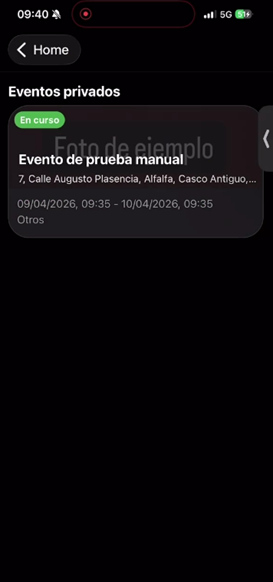
\includegraphics[width=\linewidth]{figures/paso12/eventos_priv.png}
        \caption{Eventos privados}
    \end{subfigure}
    \hspace{0.1\linewidth}
    \begin{subfigure}{0.35\linewidth}
        \centering
        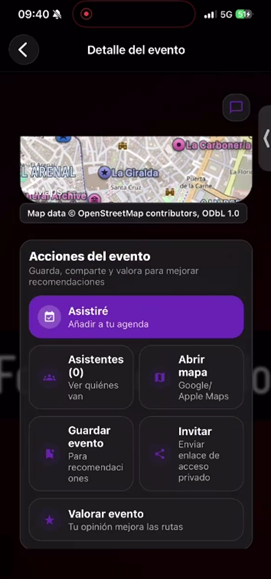
\includegraphics[width=\linewidth]{figures/paso12/det_event_priv.png}
        \caption{Evento privado}
    \end{subfigure}
    \caption{Gestión de eventos privados}
\end{figure}

\clearpage

\subsection{Mis eventos (rol de usuario)}

La sección \textit{Mis eventos} permite al creador consultar y editar las actividades que ha generado. Esta pantalla resulta útil para controlar el estado de los eventos y adaptar su configuración con el tiempo.

Dependiendo de si un evento es público o privado, y del sentido del cambio realizado, su visibilidad puede variar.
\bigskip

\textbf{Aspectos a tener en cuenta:}
\begin{itemize}[leftmargin=1.5em]

\item Cuando se edita un evento privado se mantiene visible para participantes que accedieron mediante el enlace privado y en \textit{Mis eventos}.
\item Cuando un evento pasa de público a privado deja de ser visible para todos pero se mantiene visible en \textit{Mis eventos}. Para que sea visible habría que acceder mediante el enlace privado.
\item Cuando un evento pasa de privado a público se va a moderación, desapareciendo de \textit{Mis eventos} y dejando de ser visible para las personas que habían accedido mediante el enlace y pasaría a ser visible para todos si se aprueba.
\item Cuando se edita un evento público pasa a moderación, desapareciendo de \textit{Mis eventos} y dejando de ser visible para todos.
\end{itemize}

\begin{figure}[H]
    \centering
    \begin{subfigure}{0.31\linewidth}
        \centering
        
\includegraphics[width=\linewidth]{figures/paso13/menu_lateral.png}
        \caption{Menú lateral}
    \end{subfigure}
    \hspace{0.01\linewidth}
    \begin{subfigure}{0.31\linewidth}
        \centering
        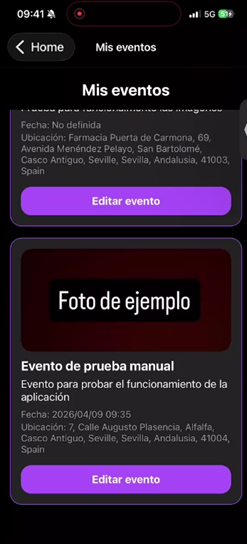
\includegraphics[width=\linewidth]{figures/paso13/mis_eventos.png}
        \caption{Mis eventos}
    \end{subfigure}
    \hspace{0.01\linewidth}
    \begin{subfigure}{0.31\linewidth}
        \centering
        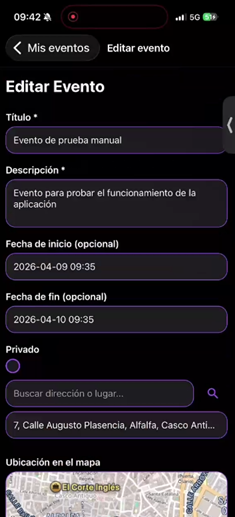
\includegraphics[width=\linewidth]{figures/paso13/editar_evento.png}
        \caption{Editar evento}
    \end{subfigure}
    \caption{Eventos creados por el usuario}
\end{figure}

\clearpage

\subsection{Moderación (rol de moderador)}

El rol de moderador se encarga de revisar aquellos eventos públicos que todavía no han sido validados para su publicación. Esta funcionalidad ayuda a mantener la coherencia y fiabilidad de la plataforma.

Desde la pantalla de moderación pueden consultarse los eventos pendientes, editarlos si fuera necesario y aprobarlos o rechazarlos. Una vez aprobados, los eventos pasan a ser visibles para el resto de usuarios.

\bigskip

\textbf{Credenciales de prueba:}
\begin{itemize}[leftmargin=1.5em]
\item Email: \texttt{mod@demo.com}
\item Contraseña: \texttt{moderator}
\end{itemize}

\begin{figure}[H]
    \centering
    \begin{subfigure}{0.31\linewidth}
        \centering
        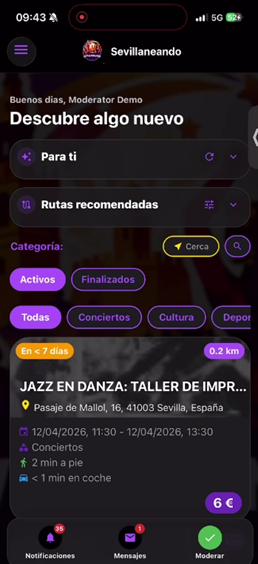
\includegraphics[width=\linewidth]{figures/paso14/pagina_principal.png}
        \caption{Página principal}
    \end{subfigure}
    \hspace{0.01\linewidth}
    \begin{subfigure}{0.31\linewidth}
        \centering
        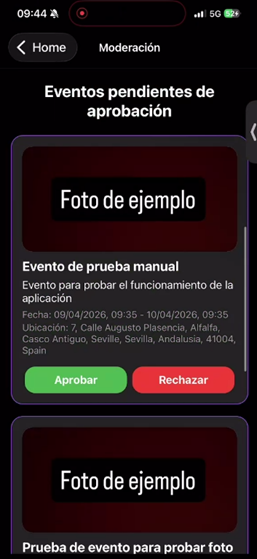
\includegraphics[width=\linewidth]{figures/paso14/moderacion.png}
        \caption{Moderación}
    \end{subfigure}
    \hspace{0.01\linewidth}
    \begin{subfigure}{0.31\linewidth}
        \centering
        
\includegraphics[width=\linewidth]{figures/paso14/editar_evento.png}
        \caption{Editar evento}
    \end{subfigure}
    \caption{Moderación de eventos}
\end{figure}

\clearpage

\subsection{Notificaciones (todos los roles)}

Las notificaciones permiten al usuario recibir información relevante sin necesidad de revisar manualmente el estado de sus eventos o actividades. Estas notificaciones pueden referirse a la aprobación o rechazo de un evento creado, recordatorios previos a la celebración de una actividad o eventos cercanos según la ubicación. Al entrar salen marcadas como nuevas y se pueden pulsar para cambiar su estado y se pueden eliminar mediante el botón.

Este sistema mejora la comunicación entre la plataforma y el usuario, y contribuye a mantener una experiencia más activa y personalizada.

\begin{figure}[H]
    \centering
    \begin{subfigure}{0.4\linewidth}
        \centering
        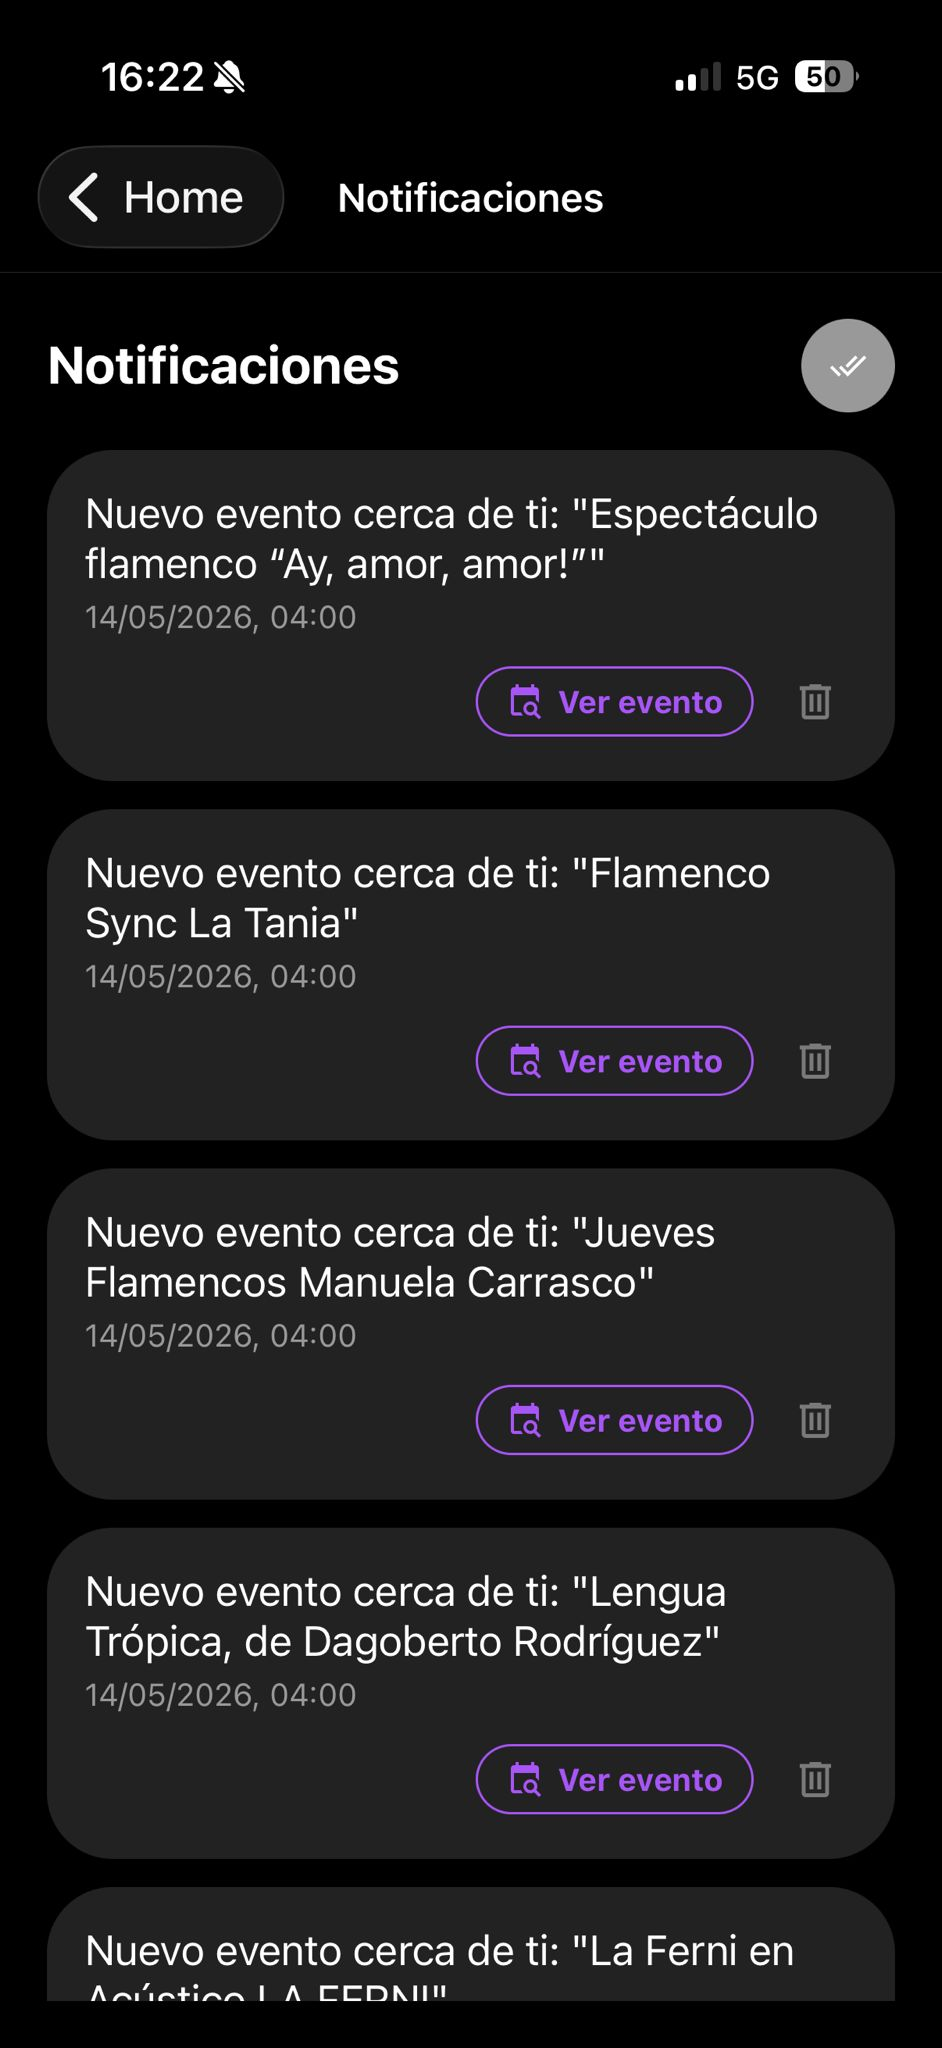
\includegraphics[width=\linewidth]{figures/paso15/notificaciones.png}
    \end{subfigure}
    \caption{Notificaciones}
\end{figure}

\clearpage

\subsection{Mensajería privada (todos los roles)}

Además del chat asociado a eventos, la aplicación incorpora mensajería privada entre usuarios. Esta funcionalidad permite establecer conversaciones directas pulsando el usuario en el chat del evento o en los asistentes. Se podrán enviar mensajes, imágenes y si se dejan pulsados estos, se podrán eliminar.

Las conversaciones privadas pueden consultarse posteriormente desde la sección de mensajes, favoreciendo la continuidad del contacto entre usuarios.

\begin{figure}[H]
    \centering
    \begin{subfigure}{0.305\linewidth}
        \centering
        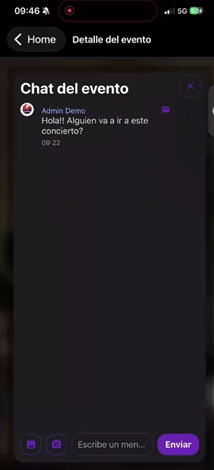
\includegraphics[width=\linewidth]{figures/paso16/chat_evento.png}
        \caption{Chat del evento}
    \end{subfigure}
    \hspace{0.02\linewidth}
    \begin{subfigure}{0.31\linewidth}
        \centering
        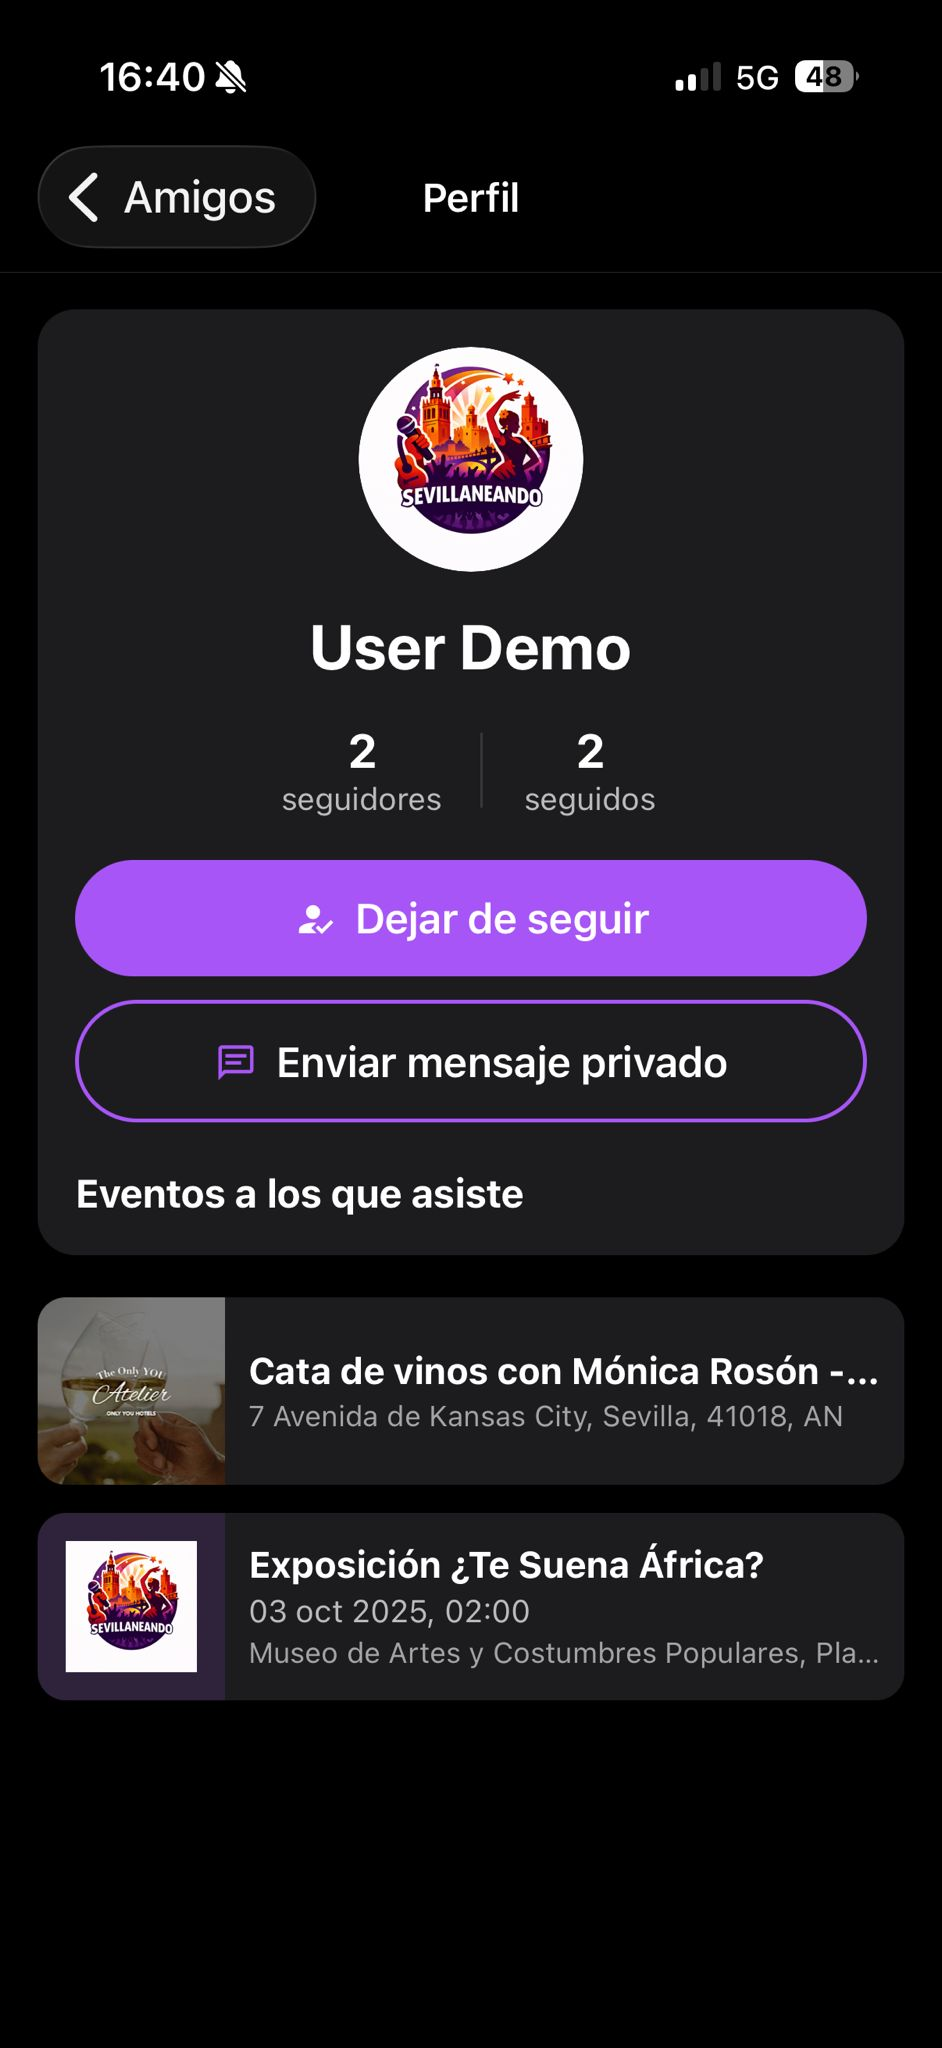
\includegraphics[width=\linewidth]{figures/paso16/ver_perfil.png}
        \caption{Ver perfil}
    \end{subfigure}
    \hspace{0.02\linewidth}
    \begin{subfigure}{0.306\linewidth}
        \centering
        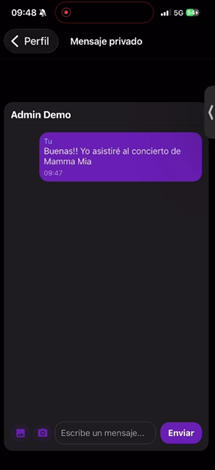
\includegraphics[width=\linewidth]{figures/paso16/chat_priv.png}
        \caption{Chat privado}
    \end{subfigure}
    \caption{Mensajes privados}
\end{figure}

\begin{figure}[H]
    \centering
    \begin{subfigure}{0.358\linewidth}
        \centering
        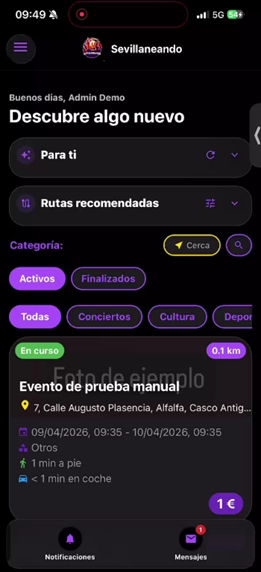
\includegraphics[width=\linewidth]{figures/paso16/pag_ppal.png}
        \caption{Página principal}
    \end{subfigure}
    \hspace{0.02\linewidth}
    \begin{subfigure}{0.373\linewidth}
        \centering
        
\includegraphics[width=\linewidth]{figures/paso16/mensajes.png}
        \caption{Mensajes}
    \end{subfigure}
    \caption{Consulta de mensajes privados}
\end{figure}

\clearpage

\subsection{Eventos finalizados}

Los eventos finalizados continúan siendo visibles dentro de la aplicación como parte del historial consultable, pero presentan restricciones respecto a las acciones disponibles. En estos casos, el usuario puede acceder a la información del evento, pero no realizar nuevas inscripciones.

Esta distinción permite preservar la utilidad informativa del sistema sin confundir al usuario sobre la disponibilidad real de cada actividad.

\begin{figure}[H]
    \centering
    \begin{subfigure}{0.4\linewidth}
        \centering
        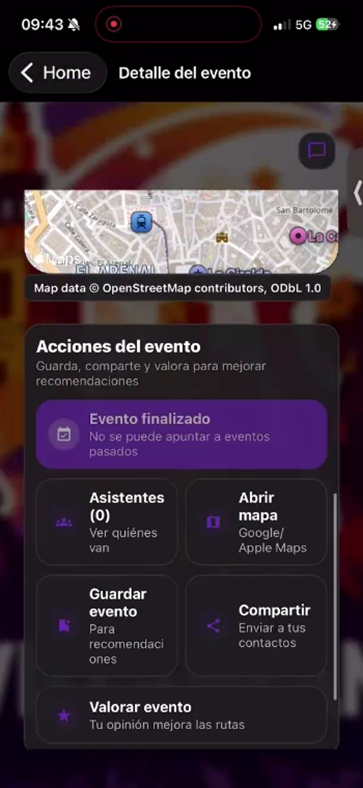
\includegraphics[width=\linewidth]{figures/paso17/evento_fin.png}
    \end{subfigure}
    \caption{Evento finalizado}
\end{figure}

\clearpage

\section{Grafo de navegabilidad}

Con el fin de complementar la guía de uso, se recomienda incluir un grafo de navegabilidad que muestre las principales pantallas de la aplicación y las rutas de transición más habituales entre ellas. Este diagrama ayuda a comprender la estructura general del sistema y la manera en que el usuario se desplaza por sus distintos módulos.

\begin{figure}[H]
    \centering
    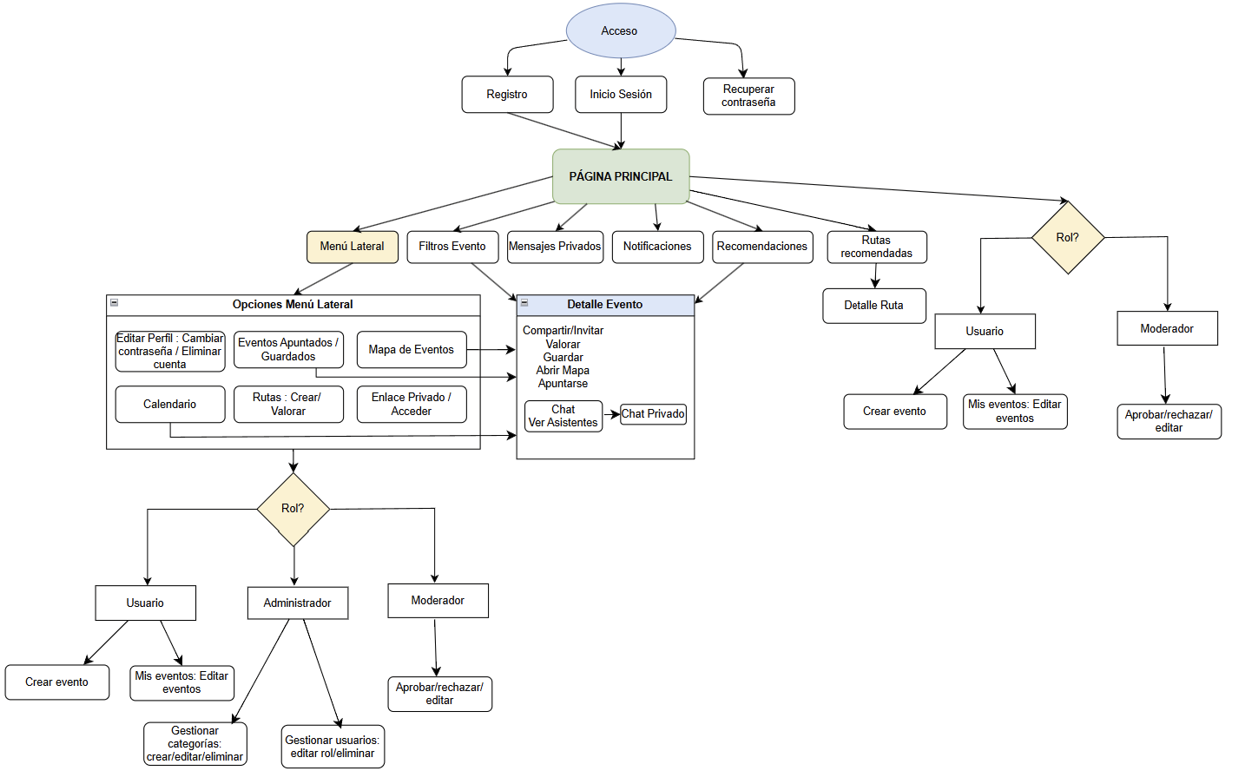
\includegraphics[width=\linewidth,height=0.99\textheight,keepaspectratio]{figures/grafo_navegacion.png}
    \caption{Grafo de navegabilidad de la aplicación}
\end{figure}

\section{Errores frecuentes}

A continuación se recogen algunos problemas habituales que pueden producirse durante el uso de la aplicación, junto con una posible explicación:

\begin{itemize}[leftmargin=1.5em]
\item \textbf{No aparecen eventos en el mapa.} Puede deberse a que el usuario no ha definido una ubicación en el perfil.
\item \textbf{No llegan notificaciones de eventos cercanos.} Puede ser necesario revisar los permisos de ubicación.
\item \textbf{No es posible apuntarse a un evento.} Es posible que el evento se encuentre finalizado o no admita nuevas inscripciones.
\item \textbf{No se puede compartir un evento privado libremente.} En este tipo de eventos la capacidad de invitación queda restringida al creador.
\item \textbf{Las recomendaciones no resultan relevantes.} El sistema mejora sus propuestas a medida que el usuario interactúa con la aplicación.
\item \textbf{No se visualizan correctamente algunas funciones basadas en proximidad.} Debe comprobarse que la ubicación del perfil está configurada correctamente.
\end{itemize}
